

\section{Time Delay Cosmology}

Time Delay Cosmology is an eeffect related to lensing, in particular strong lensing effect, where we have multiple images of the same source, which are time delayed due to two effects: the different paths of the light rays and the general relativistic effect, called the Shapiro (1964) delay, owing to the difference in gravitational potential experienced by the photons along the paths. This effect is possible only if there is a time-varyiable source.

\begin{figure}[H]
    \centering
    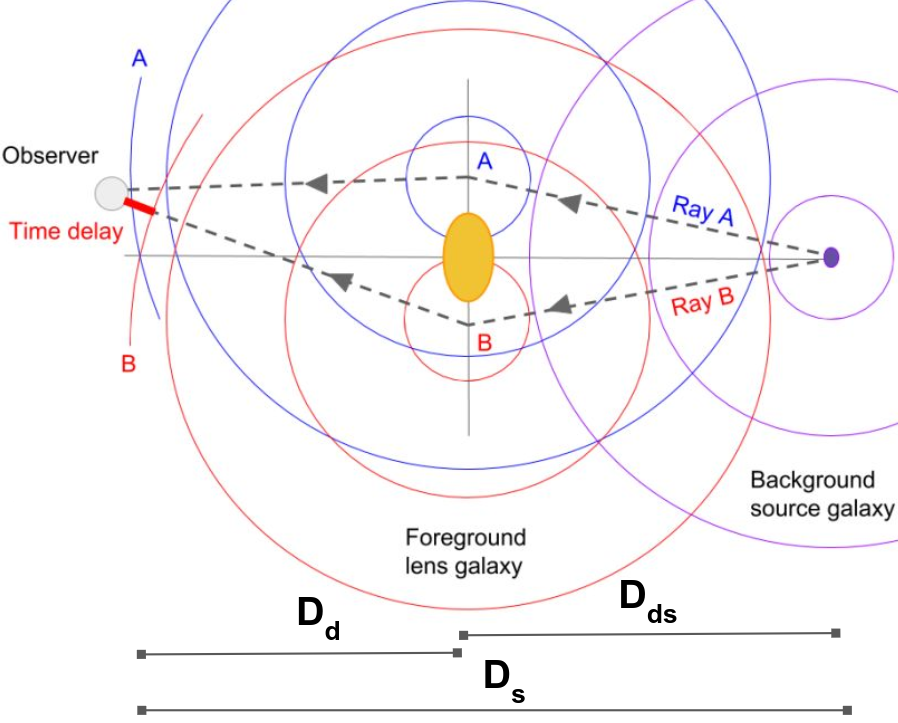
\includegraphics[width=0.7\textwidth]{assets/time_delay.png}
    \caption{Time delay cosmology}
\end{figure}

The time delay between image A and image B is given by:
$$
    \Delta \tau_{AB} = \frac{D_{\Delta t}}{c} \, \Delta \Phi_{AB}
$$
$$
    D_{\Delta t} \equiv (1 + z_d) \frac{D_d D_s}{D_{ds}}
$$

where $\Delta \Phi$ is the Fermat potential difference between the two image positions. It can be predicted given a model for the mass distribution of the lens, along with the deflection angle:
$$
    \phi = \frac{1}{2}(\theta - \beta)^2 - \psi(\theta)
$$
Here, the first term corresponds to the \textbf{geometrical delay}, and $\psi(\theta)$ is the lens potential responsible for the \textbf{Shapiro delay}.

Steps:
\begin{enumerate}
    \item \textbf{Measure the time delay between the two images}: 
    
    The basic idea is to detect variations in the brightness of the quasar images in a lens system and use these variations to determine the time delay between the multiple images, given that the intrinsic brightness variations of the quasar manifest in each of the multiple images

    \item \textbf{Measure and model the potential}
    \item \textbf{Infer the time delay distance $D_{\Delta t}$}
    \item \textbf{Convert it into cosmological parameters}
\end{enumerate}

\subsubsection{Time Delay Cosmograhpy with Supernovae}

%todo: check and enhnance this

Multiply-imaged supernovae provide an independent way to measure the Hubble constant $H_0$. Precise modeling of the lensing mass distribution and accurate estimation of the time delays between the images are essential to extract cosmological constraints from these systems.

So far, only a few multiply-imaged supernovae have been found (e.g., Refsdal, H0pe, SN Encore). A notable case is the supernova observed in the lensing galaxy cluster MACS J0138.0--2155. As illustrated in the figure, a combination of lens modeling and measured time delays can be used to obtain tight constraints on $H_0$ from such supernovae.

Remarkably, a sibling to SN Encore (SN "Requiem") was discovered in the same host galaxy, making the MACS J0138.0-2155 cluster the first system known to produce more than one observed multiply-imaged SN. SN Requiem has a fourth image that is expected to appear within a few years, providing an unprecedented decade-long baseline for time-delay cosmography. The fourth image of SN Requiem is expected to appear:

\begin{itemize}
    \item For $H_0 = 73 km/s/Mpc$, in late 2026
    \item For $H_0 = 67 km/s/Mpc$, in mid 2027
\end{itemize}

The long time delays of the next-appearing SN Requiem and SN Encore images provide excellent opportunities to measure H0 with 2-3\% uncertainty.

\subsection{Statistical properties of LSS}

\subsubection{Lyman-$\alpha$ forest}

Absorption spectra of distant luminous quasars (QSOs) provide a powerful way to probe the intergalactic medium (IGM) at high redshift, through the analysis of the so-called \textbf{Lyman-$\alpha$ forest}.

The UV light emitted by a distant quasar, at wavelengths bluewards of the Ly-$\alpha$ emission line ($\lambda < 1216\,$\AA), travels through the IGM and can be absorbed by intervening clouds of neutral hydrogen. Due to cosmic expansion, photons are redshifted into resonance with the Ly-$\alpha$ transition at different points along the line of sight. This results in a series of absorption features—known as the Ly-$\alpha$ forest—seen in the quasar spectrum at observed wavelengths
$$
\lambda_{\text{obs}} = 1216\,\text{\AA}\ \times\ (1 + z_a),
$$
where $z_a$ is the redshift of the absorbing cloud.

The Ly-$\alpha$ forest traces the distribution of neutral hydrogen in the IGM, which in turn is a \textit{biased tracer} of the underlying dark matter distribution. By studying the clustering statistics of the transmitted flux, we can constrain both the shape and amplitude of the matter power spectrum and therefore measure the growth of large-scale structure at redshifts $2 < z < 6$. This redshift range is inaccessible to other LSS probes, such as cosmic shear or galaxy clusters.

The fluctuations of the Ly α forest flux,
𝛿f = F(x)/<F(x)> -1, along the line of sight
L, can be used to measure the
one-dimensional (1D) Ly-α forest power
spectrum:

$$
P_F(k) \equiv \dfrac {\mid \bar \delta_f(k) \mid^2}{L}
$$

Cosmological inference from the Ly-$\alpha$ forest spectra is complicated by there being \textbf{no reliable analytic model for the mildly nonlinear densities probed by the forest}. All analyses require a comparison with large cosmological simulations.

\subsubsection{21cm Line}

21-cm radiation originates from the \textbf{hyperfine transition} (spin-flip) of the hydrogen atom:
\begin{itemize}
    \item Strongly forbidden line, $t_{1/2} \sim 10^7$ yr
    \item HI very abundant
    \item Spectrally isolated
    \item Small obscuration
    \item Earth's atmosphere is transparent to radio frequencies
\end{itemize}

Assuming that the hydrogen atoms are uniformly distributed throughout galaxies, each line of sight through the galaxy will reveal a hydrogen line. The only difference between each of these lines is the \textbf{Doppler shift} that each of these lines has.

Observations of the hydrogen line have been used to reveal the \textbf{spiral shape} of the Milky Way and to calculate the \textbf{mass and dynamics of individual galaxies} through their velocity rotation curves.

\subsection{Intensity Mapping}

\textbf{Intensity mapping} is an observational technique for surveying the large-scale structure of the universe by using the integrated radio emission from unresolved HI gas clouds. The frequency of the emission line is redshifted by the expansion of the Universe, thus the signal can be used to reconstruct the matter density field over cosmic time (\textit{tomography}). 

Intensity mapping surveys can be carried out much faster than conventional optical redshift surveys; it is possible to map significantly larger volumes of the Universe.

It can be used to probe the cosmological ``dark ages'' from recombination (when stable hydrogen atoms first formed) to reionization:
\begin{itemize}
    \item It can provide a picture of how the universe was re-ionized: neutral hydrogen which has been ionized by radiation from stars or quasars will appear as holes in the 21 cm background.
    \item By mapping the intensity of redshifted 21~cm radiation --- $A = 21\,\mathrm{cm} \times 142$ --- it can measure the matter power spectrum in the period after recombination (BAO, RSD, etc).
\end{itemize}

\begin{figure}[H]
    \centering
    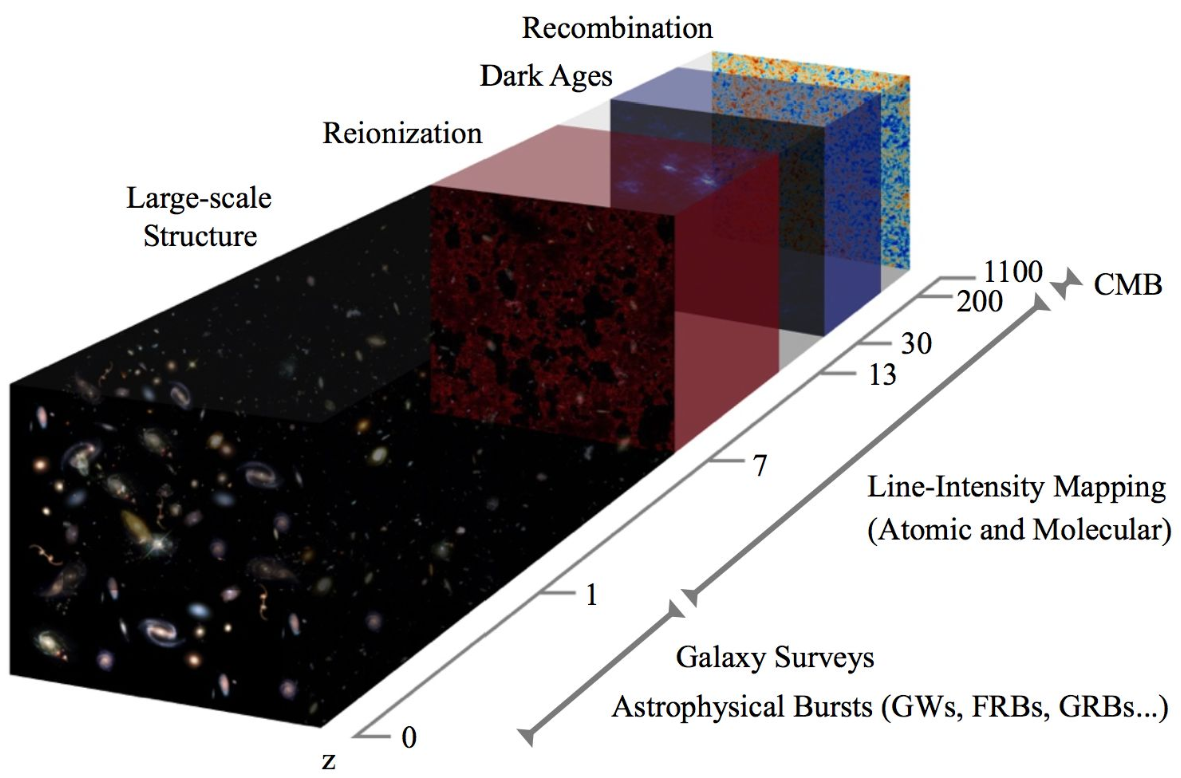
\includegraphics[width=0.7\textwidth]{assets/21-cm-if.png}
    \caption{21-cm intensity mapping}
\end{figure}

\missing{slide 17}

\begin{observationblock}[Square Kilometer Array Observatory (SKAO)]
The Square Kilometer Array Observatory (SKAO) is a next-generation radio telescope project designed to perform wide and deep surveys of the sky using thousands of antennas in both Africa and Australia. The SKA will map large-scale structure via HI 21-cm intensity mapping over a wide redshift range ($0.35 < z < 6$), providing galaxy and intensity maps with unprecedented sensitivity and area coverage. Its two main components, SKA1-mid (South Africa) and SKA1-low (Australia), target different frequency ranges and science cases.
\begin{itemize}
    \item \textbf{Wide survey:} Covers 20,000 deg$^2$ at $0.35$--$1.05$ GHz for galaxy and HI intensity mapping ($0.35 < z < 3$).
    \item \textbf{Deep survey:} Covers 100 deg$^2$ at $200$--$350$ MHz for HI intensity mapping at higher redshift ($3 < z < 6$).
\end{itemize}
\end{observationblock}

\subsubsection{21-cm challenges}

The IM signal is weak compared to the \textbf{contaminants}:
\begin{itemize}
    \item \textbf{Receiver noise:} Amplitude comparable to signal~$\to$ isotropic, 1/$f$ noise can be removed, manageable in power spectrum space.
    \item \textbf{Instrumental errors:} Calibration uncertainties, sidelobes, pointing errors, polarization leakage.
    \item \textbf{Radio Frequency Interference (RFI):} Contaminates in spatial and frequency space~$\to$ go to the desert, stay away from satellites.
    \item \textbf{Foreground contaminations:} Galactic emission and extra-Galactic point sources.
\end{itemize}

\section{Cosmology with Gravitational Waves}

Most of what we know about the Universe is through photons. Lots of ongoing efforts to obtain information about the universe using \textbf{non-EM cosmic messengers}: neutrinos, gravitational waves, cosmic rays, etc.

\subsection{Cosmic Neutrinos}

The IceCube Neutrino Observatory, located at the South Pole, is designed to detect high energy (≳1 TeV) astrophysical neutrinos and identify their sources. \textbf{Neutrinos are detected through Cherenkov radiation, emitted by charged secondary particles that are produced by neutrino interactions with nuclei in the ice or bedrock}. Because of the large momentum transfer from the incoming neutrino, the directions of secondary particles are closely aligned with the incoming neutrino direction, enabling the identification of the neutrino's origin

cosmic neutrinos observed from the north pole have high energy, most of them are expected to be from blazars.

\todo{finish this section}

\subsection{Gravitational Waves}

General Relativity predicts that space-time perturbations propagate through empty space at the speed of light.

Two possible polarizations:

\begin{figure}[H]
    \centering
    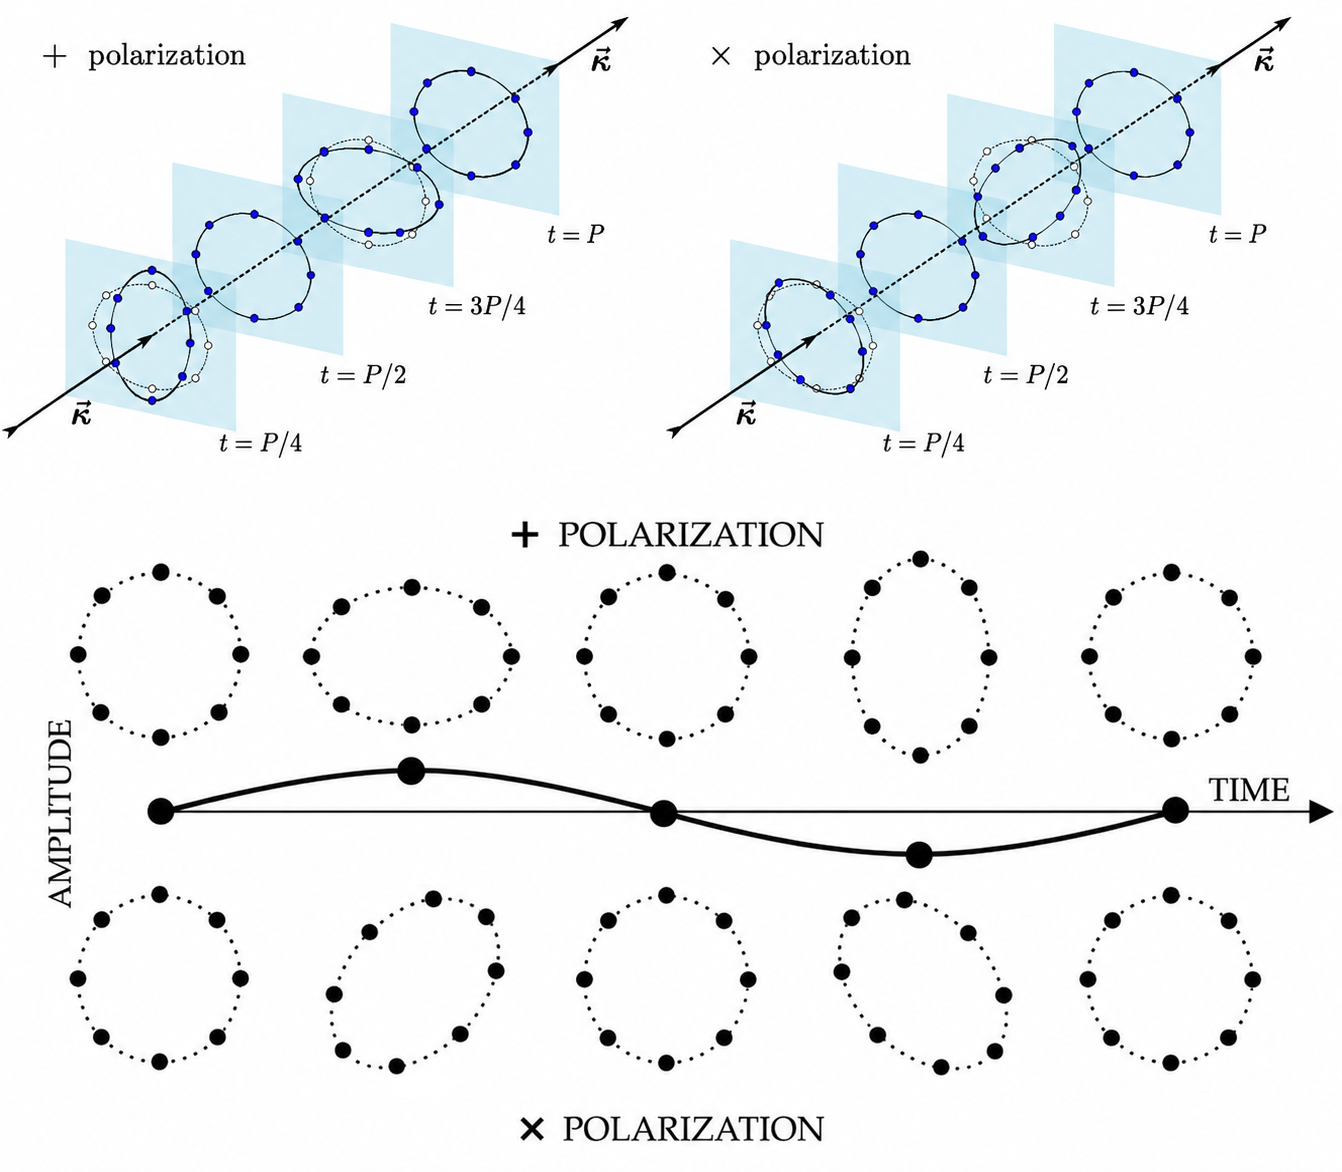
\includegraphics[width=0.7\textwidth]{assets/grav_waves.png}
    \caption{Gravitational waves polarizations}
\end{figure}

\begin{observationblock}[First indirect evidence of GW]
    \begin{minipage}{0.6\textwidth}
    PSR B1913+16: First indirect evidence from orbital period decay of binary system composed of a neutron star and pulsar, a rapidly rotating, highly magnetized neutron star (1993 Nobel prize J. Taylor, R. Hulse): the orbital decay match the energy loss predicted from GR due to gravitational wave radiation.
    \end{minipage}%
    \hfill
    \begin{minipage}{0.38\textwidth}
        \centering
        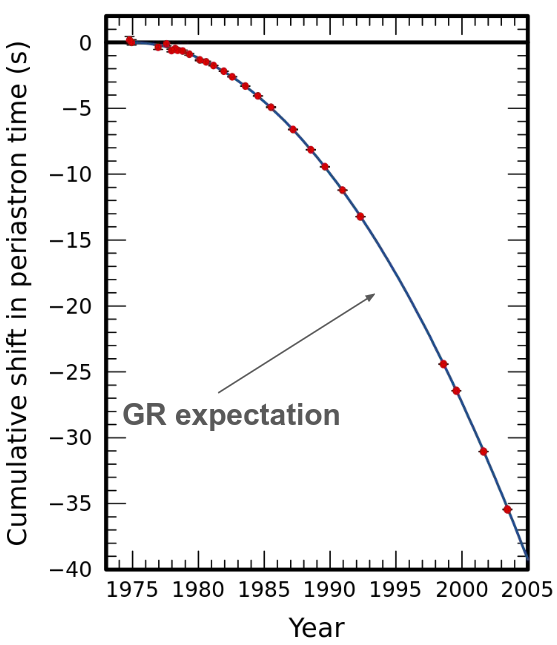
\includegraphics[width=\textwidth]{assets/gw_first.png}
        \captionof{figure}{Orbital decay vs GR prediction}
    \end{minipage}
\end{observationblock}

\subsubsection{Gravitational Wave Interferometers}

Gravitational wave astronomy has dramatically expanded our understanding of the masses of compact stellar remnants (black holes and neutron stars) by allowing precise measurements of merging objects.

For a binary system, the wave's freq sweep and amplitude (strain) depend on $\mathcal{M} = (m_1 m_2)^{3/5} / (m_1 + m_2)^{1/5}$, and luminosity distance $D_L$:

$$
\begin{array}{rl}
\dfrac{d\Omega}{dt} &\propto \left( \dfrac{G \mathcal{M}}{c^3} \right)^{5/3}
\\
h &\propto \dfrac 1{D_L} \left( \dfrac{G \mathcal{M}}{c^3} \right)^{5/3} \Omega^{2/3}
\end{array}
$$

Dimensionless strain, h= 𝜟l/l, is the main observable measured; the typical relative deformation:
$$
h = \dfrac{\Delta l}{l} \sim 10^{-21}
$$

\begin{exampleblock}[LIGO strain]
E.g. for Laser Interferometer Gravitational-Wave Observatory (LIGO), the typical relative deformation is: $l \sim 4km \to \Delta l \sim 10^{16} cm$.
\end{exampleblock}

\missing{... first detection (2015) ...}

\begin{figure}[H]
    \centering
    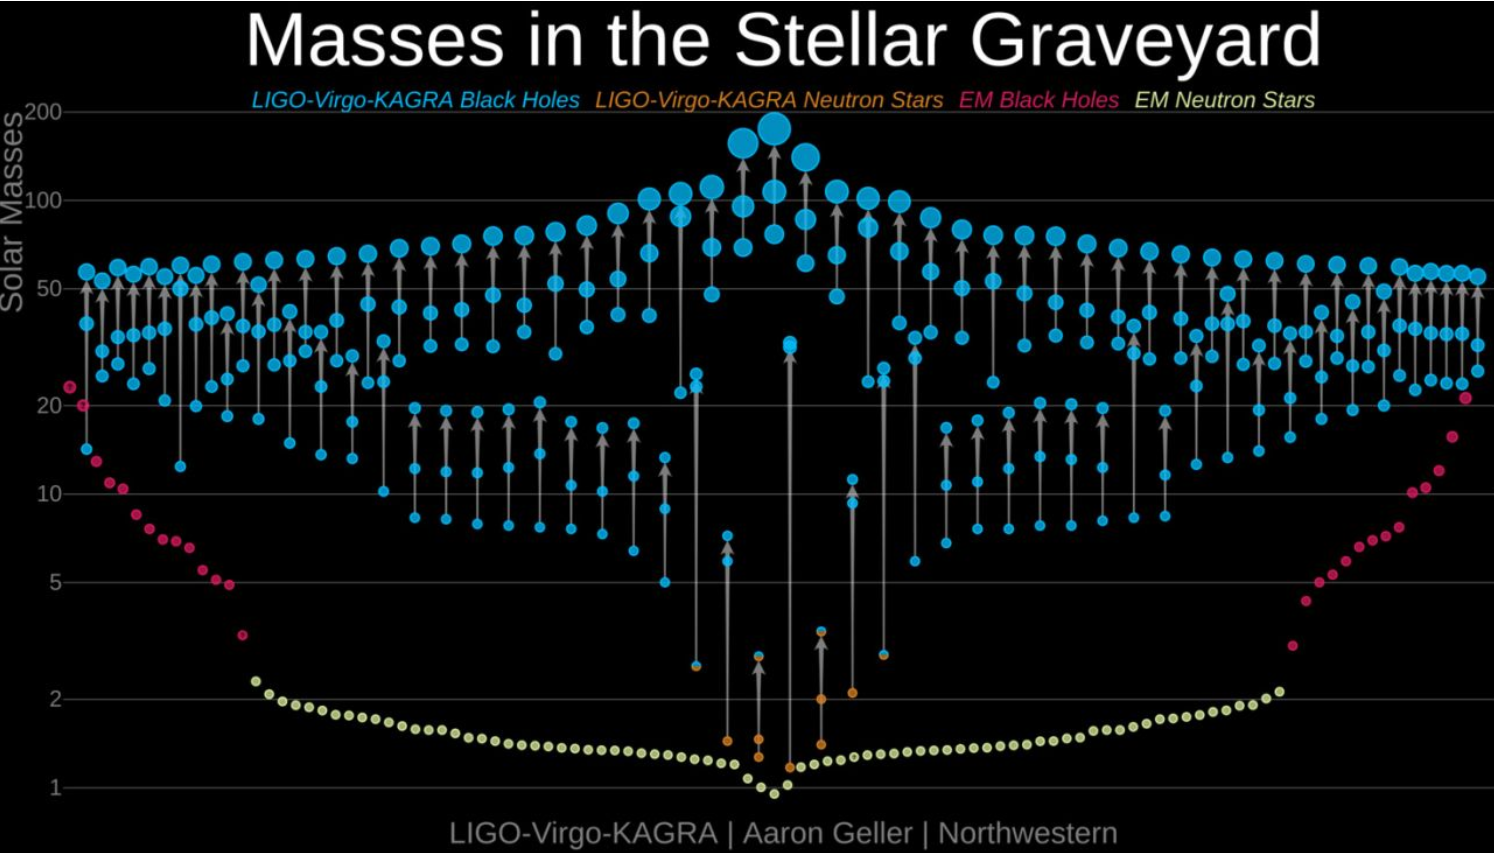
\includegraphics[width=0.8\textwidth]{assets/gw_obs.png}
    \caption{Remnant masses observed via gravitational wave (GW) detections (LIGO-Virgo-KAGRA) compared to those previously inferred from electromagnetic (EM) observations}
\end{figure}

One major insight from GW observations is the identification, and partial resolution, of \textbf{two mass gaps} that were believed to exist between neutron stars and black holes:

\begin{itemize}
    \item \textbf{Lower Mass Gap (``Mass Gap''):} Prior to GW detections, EM observations seemed to suggest a dearth of compact objects between the most massive neutron stars ($\sim 2\,M_\odot$) and the lightest black holes ($\sim 5\,M_\odot$)...
    \item \textbf{Upper Mass Gap (``Pair-Instability Gap''):} Stellar evolution theory predicts a scarcity of black holes with masses above $\sim 150 M_\odot$...
\end{itemize}

\missing{first Binary neutron star merger, virgo didn't detect it due to the direction of the signal}

\missing{triangulation of the GW signal}

\subsection{Standard sirens}

Gravitational wave (GW) sources can serve as \textbf{``standard sirens''}—the GW analog to ``standard candles''—because the amplitude of the observed GW strain, $h$, provides a direct measurement of the luminosity distance to the source ($h \propto D_L^{-1}$). This measurement is ``self-calibrating,'' relying only on fundamental physics, without the need for external calibration (Schutz 1986).

\begin{itemize}
    \item \textbf{Self-calibrating:} The shape and evolution of the GW signal alone allow the luminosity distance, $D_L$, to be inferred with no reliance on a cosmic distance ladder.
    \item \textbf{Direct distance:} GW strain amplitude directly encodes $D_L$ to the merger event.
    \item \textbf{Redshift challenge:} However, redshift ($z$) is not directly available from the GW signal, since there are no spectral lines. If an electromagnetic (EM) counterpart is detected, it enables identification of the host galaxy, allowing $z$ to be measured, and thus the $D_L$--$z$ relation can be constructed for cosmology.
    \item \textbf{Observed mass:} The masses inferred from GW data are ``redshifted'' chirp masses: $m_{\mathrm{obs}} = m_{\mathrm{src}} (1+z)$.
\end{itemize}

\textbf{First GW standard siren: GW170817.} The binary neutron star merger GW170817 was the first GW event with an EM counterpart, which allowed the host galaxy (NGC 4993) to be identified. 
\begin{align*}
    D_L &= 44^{+3}_{-3}~\mathrm{Mpc} &\text{(from GW signal)} \\
    z_{\mathrm{NGC\ 4993}} &= 0.0098 \\
    H_0 &= 70^{+12}_{-8}~\mathrm{km\,s^{-1}\,Mpc^{-1}}
\end{align*}
Assuming the group centroid redshift for NGC 4993, these measurements yielded an independent determination of the Hubble constant, $H_0$ (see Figure).

\begin{figure}[H]
    \centering
    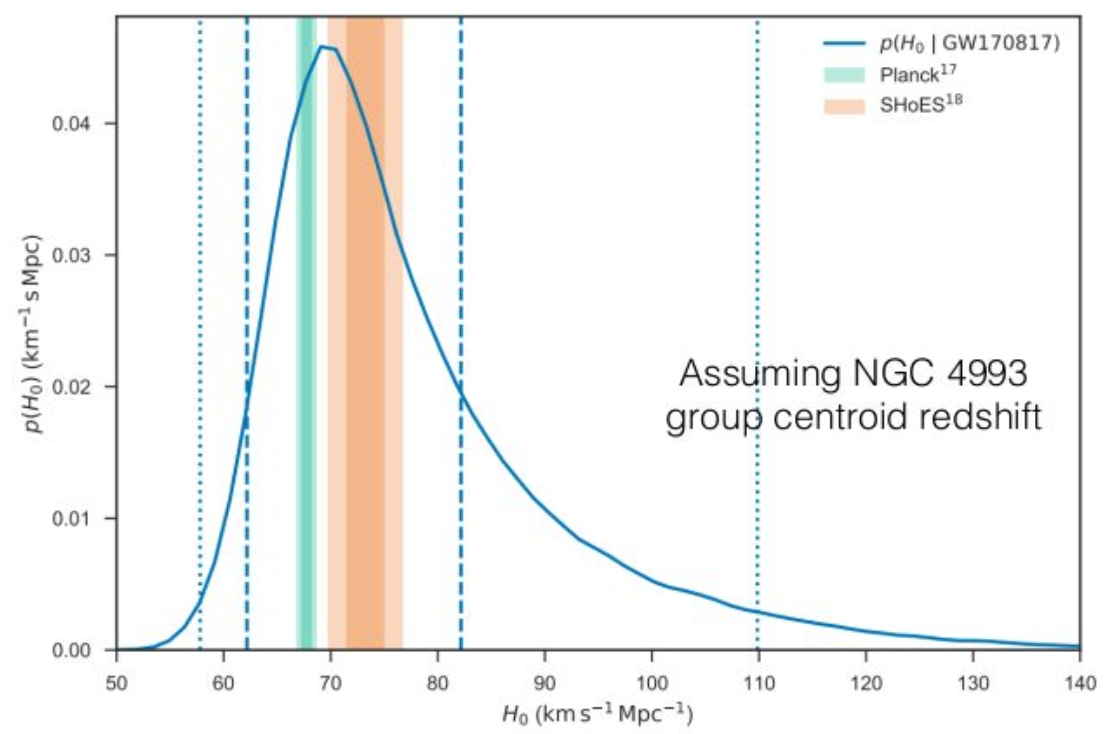
\includegraphics[width=0.7\textwidth]{assets/NGC4993.png}
    \caption{Posterior probability for $H_0$ (blue) from GW170817, with comparison to Planck (orange) and SHoES (green) results. The GW signal constrains $D_L$, the EM counterpart allows $z$, and their combination provides a direct, calibration-independent measurement of $H_0$. Figure adapted from \texttt{arxiv:1710.05835}.}
\end{figure}

This approach opens the way for an independent measurement of cosmic expansion, and as more standard siren events are observed, the constraints on cosmological parameters such as $H_0$ will become increasingly competitive with traditional (electromagnetic) methods.

\subsubsection{Dark Standard Sirens}

A \textbf{dark siren} is a gravitational wave event without EM counterpart. Most binary mergers, and in particular binary black hole (BBH) mergers, do not have associated electromagnetic counterparts. However, in the absence of such a counterpart signposting the host galaxy directly, we can still use the gravitational-wave observations to give us information about the sky position of the source - and in this way narrow down the host galaxy to a set of candidate galaxies in this region. Combining redshift information from all of these possible host galaxies then allows us to measure $H_0$ statistically.

\subsubsection{Spectral Sirens}

In this case we just rely on our astrophysical knowledge of compact object distribution in the universe:

Bright sirens require an electromagnetic counterpart to determine the redshift of the emission source while dark sirens rely on the presence of complete galaxy catalogs over large sky regions. Spectral sirens, using GW data alone, can circumvent these limitations by leveraging features in the mass distribution of compact binaries: Astrophysically motivated models for the source-frame mass distribution of black holes, can be used to statistically infer the redshift of the source and thereby breaking the mass-redshift degeneracy

\begin{figure}[H]
    \centering
    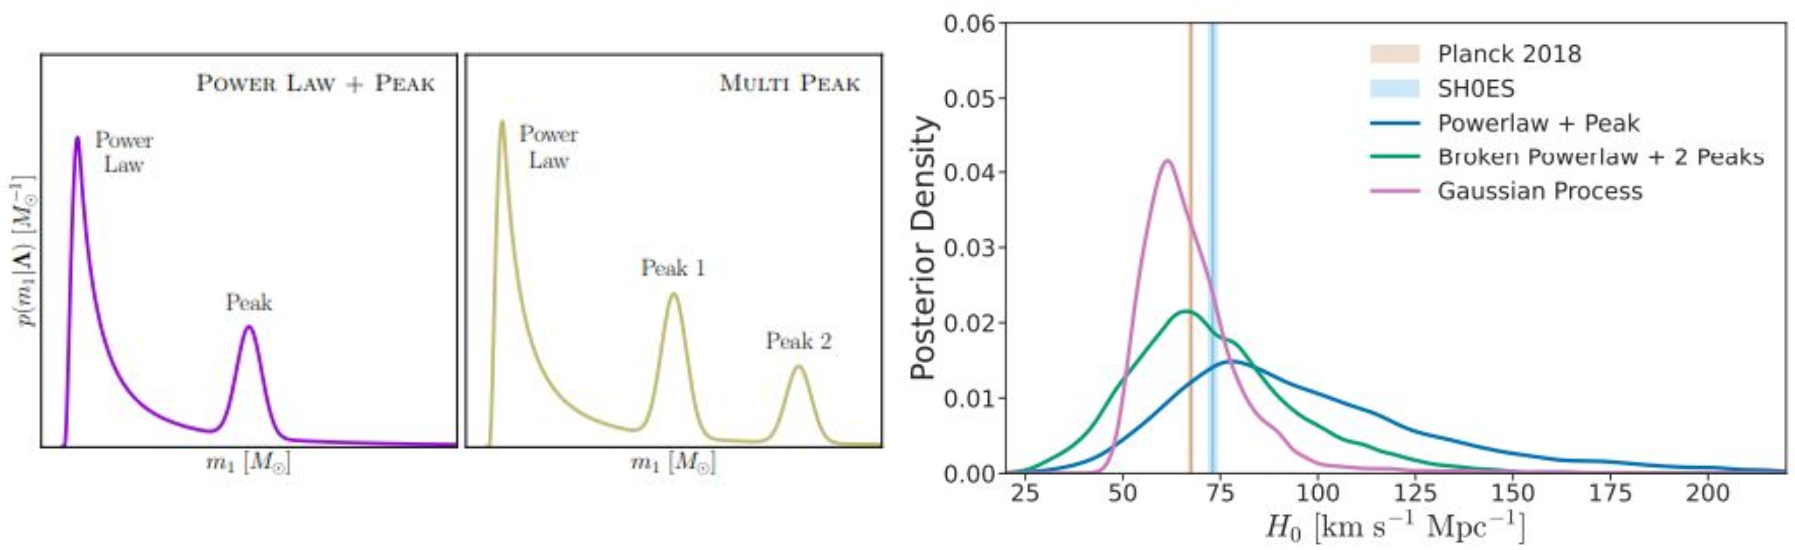
\includegraphics[width=0.7\textwidth]{assets/spectral_sirens.png}
    \caption{Left: Example models for the source-frame black hole mass distribution, including power-law and multi-peak features. Right: Posterior distributions for the Hubble constant $H_0$ from spectral siren analyses, compared to Planck and SHoES measurements. Figure adapted from \cite{Chon2022}.}
\end{figure}

\subsubsection{Dark + Spectral Sirens}

\subsubsection{Dark Standard Sirens}

\textbf{Gravitational-Wave Transient Catalog GWTC-4.0: Constraints on the Cosmic Expansion Rate and Modified Gravitational-wave Propagation} \href{https://arxiv.org/pdf/2509.04348}{https://arxiv.org/pdf/2509.04348}

Modified gravity can introduce ``GW friction'', that is a modifications to the GW amplitude received at the observer. This effect is indistinguishable from a change in the luminosity distance to the GW source. The result is that the luminosity distance $D_L^{\mathrm{GW}}$ inferred for a GW source differs from the EM luminosity distance $D_L^{\mathrm{EM}}$.

The ratio $D_L^{\mathrm{GW}} / D_L^{\mathrm{EM}}$ is thus a convenient probe of departures from GR on cosmological scales. The ratio is always equal to one in GR, and in cosmological modified--gravity models can become a function of redshift.

\begin{figure}[H]
    \centering
    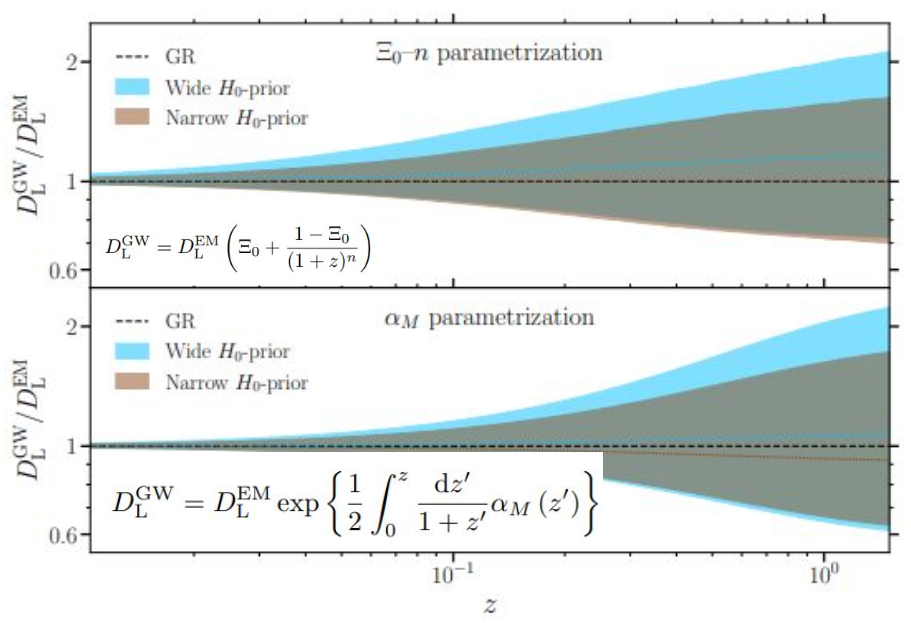
\includegraphics[width=0.7\textwidth]{assets/dark_standard_sirens.png}
    \caption{Reconstructed $D_L^{\mathrm{GW}}/D_L^{\mathrm{EM}}$ vs.\ redshift for two modified gravity models; contours show 90\% CIs, with the GR value as a dashed black line.}
\end{figure}

\subsection{Gravitational Wave Background}

\textbf{Cosmological GW background:} This is a potential signature of processes in the early Universe, such as inflation, preheating, and reheating, which could leave imprints in the GW spectrum across a broad frequency range ($10^{-18}$--$10^{8}$~Hz). For example, first-order phase transitions in the early Universe could produce a narrow-band GW feature peaking at $10^{-12}$~Hz, along with a broadband component in the band $10^{-5}$--$1$~Hz. Other sources include cosmic strings, which can generate GWs across an extremely wide frequency range ($10^{-10}$--$10^{10}$~Hz), and a variety of alternative cosmological scenarios.

\textbf{Astrophysical GW background:} An astrophysical GW background could arise from the superposition of a large number of unresolved sources since the beginning of stellar activity. Detecting this background would provide constraints on compact object physics, the initial mass function (IMF), and the star formation history, thus probing the Universe at redshifts $z \sim 0.02$\textendash 10. However, from the perspective of searching for a primordial cosmological background, the astrophysical background acts as a ``noise'' source, potentially masking or contaminating the relic cosmological GW signal.

\begin{figure}[H]
    \centering
    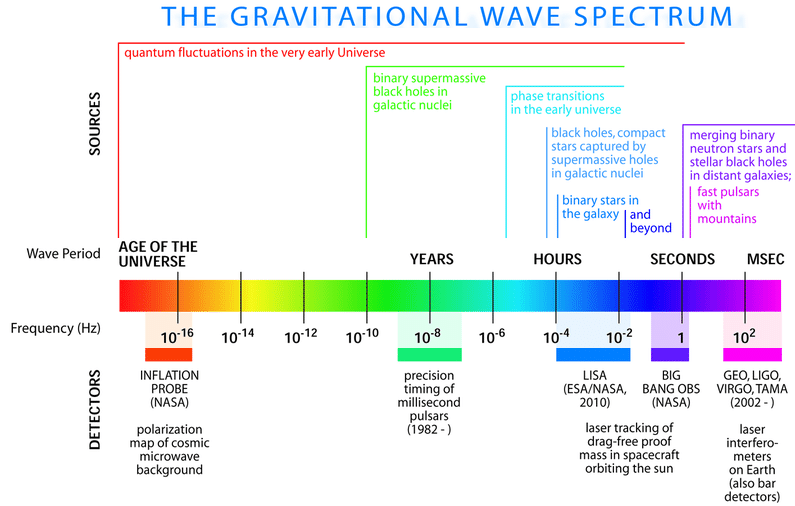
\includegraphics[width=0.7\textwidth]{assets/gw_spectrum.png}
    \caption{The gravitational wave spectrum: sources and detectors across frequency bands.}
\end{figure}

\subsubsection{Pulsars as GW detectors}

Not all pulsars are equally suited for high-precision timing applications such as pulsar timing arrays (PTAs). PTAs use the remarkable regularity of pulse arrival times from selected pulsars to search for and characterize the gravitational wave background, but only a special class of pulsars—known as recycled or millisecond pulsars—combine the rotational stability, short pulse periods, and longevity required for this task.

\begin{itemize}
    \item \textbf{Ordinary pulsars:} There are roughly 3350 ordinary pulsars known, typically with long pulse periods and significant rotational irregularities (timing noise). Their characteristic ages are less than $10^7$ years. These features render them unsuitable for high-precision timing (see red region in Figure).
    \item \textbf{Recycled (millisecond) pulsars:} There are about 500 known recycled pulsars, which have been spun up ('recycled') in binary systems. These are the most rapidly rotating pulsars, with spin periods in the millisecond range, and their characteristic ages exceed $10^9$--$10^{10}$ years. They exhibit remarkably stable rotation and short pulses, making them ideal for high-precision timing.
\end{itemize}

\begin{observationblock}[Precision of millisecond pulsars]
The periods of the best-timed millisecond pulsars can be measured to astonishing precision. E.g., on January 16, 1999, the period of PSR~J0437$-$4715 was measured as:
$$
P = 5.757451831072007~\mathrm{ms} \pm 0.000000000000008~\mathrm{ms}
$$
\end{observationblock}

Performing repeated observations of the Times of Arrival (ToAs) at the telescope of the pulsations from a given pulsar and searching the ToAs for systematic trends on many different timescales, from minutes to decades.

The key quantities are the \textbf{residuals}: The $i$-th residual $r_i$ is the difference in spin phase $\Phi$ between the observed phase of arrival of the $i$-th pulse and the phase of arrival of that pulse as predicted by the model:
$$
r_i = \phi_{\mathrm{observed}, i} - \phi_{\mathrm{model}, i}
$$

\subsubsection{Pulsar Timing Array}

Using a number of pulsars distributed across the sky it is possible to separate the timing noise contribution from each pulsar from the signature of the GW background, which manifests as a local (at Earth) distortion in the times of arrival of the pulses which is common to the signal from all pulsars.

There are different effects that can cause similar changes in the timing of many pulsars at once. By looking at the pattern of these changes, we can figure out what caused them:

\begin{itemize}
    \item \textbf{Clock errors:} If the clock on Earth has an error, it affects all measured times in the same way. This means every pulsar will show exactly the same change in the arrival times. This is called a \textbf{monopole} signature.

    \item \textbf{Solar-System ephemeris errors:} If our calculation of the position of the Solar System is off, the error will be bigger for some pulsars and smaller for others, depending on their position in the sky. This creates a pattern called a \textbf{dipole} signature.

    \item \textbf{Gravitational wave background:} A gravitational wave background makes a different, characteristic pattern in the timing data. It creates a pattern across the sky known as a \textbf{quadrupole} signature---this is the unique fingerprint searched for by PTAs when looking for gravitational waves.
\end{itemize}

\subsubsection{GW background due to Super Massive Black-Hole Binaries (SMBHBs)}

Current paradigm is that:

Mergers are an essential part of galaxy formation and evolution. The nuclei of most (possibly all) large galaxies host massive black holes (MBHs) with masses $M \gtrsim 10^6~M_\odot$. When such MBHs form a binary system, and their orbital separation $a$ shrinks to less than about 1~pc, gravitational wave (GW) emission at frequency $f$ becomes the dominant process driving energy loss. This causes the MBH binary to inspiral and shrink even more rapidly.

The frequency of the GWs emitted by a MBH binary is given by:
$$
f \sim 3~\mathrm{nHz} \left[ \frac{M}{10^9 M_\odot} \right]^{1/2} \left[ \frac{a}{0.01~\mathrm{pc}} \right]^{-3/2}
$$
which is in the nanohertz range, and depends on the mass of the MBHs and the orbital separation.

\subsubsection{Expected vs observed Strain Spectrum of GWB}

\todo{check this section}

In the simplest scenario, the expected amplitude spectrum from the ensemble of supermassive black hole (MBH) binaries (assumed isotropic and stochastic) follows:
$$
h_c(f) \sim f^{-\alpha} \quad \text{with} \quad \alpha = 2/3
$$
where $h_c(f)$ is the characteristic strain amplitude at frequency $f$.

With a ``strain'' amplitude $h_c$ theoretically expected in a broad range:
$$
h_c \approx 6 \times 10^{-17} \text{~to~} 8 \times 10^{-15}
$$
around the frequency $f_{\mathrm{GW}} = 1~\mathrm{yr}^{-1}$.

In terms of the time-domain power spectrum $P(f)$ of the timing residuals, this leads to:
$$
P(f) \propto \frac{h_c^2(f)}{f^3} = f^{-3} \cdot f^{-4/3} = f^{-13/3}
$$

\begin{figure}[h]
    \centering
    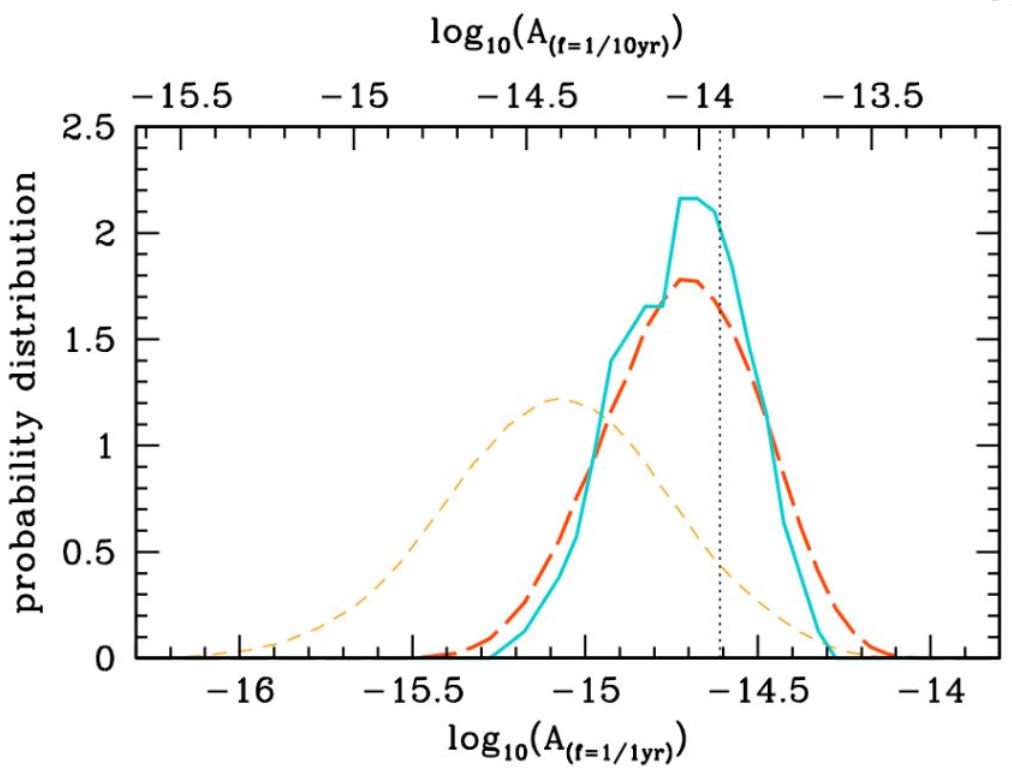
\includegraphics[width=0.5\textwidth]{assets/gwb_strain_spectrum.png}
    \caption{(Left) The expected amplitude spectrum for the gravitational wave background (GWB) from MBH binaries follows a power law with $\alpha = 2/3$. (Right) Several recent calculations of the strain amplitude and distribution. See references in the text for details.}
\end{figure}

\missing{observed strain spectrum}

A number of processes (potentially) occurring in the early Universe can also produce a stochastic GWB at nanohertz frequencies.

key discriminants compared to SMBH Background:

\begin{itemize}
    \item Spectral shape
    \item Gaussianity/burstiness
    \item possible anisotropies or polarization
    \item the presence of narrow spectral lines
\end{itemize}